\documentclass[12pt]{article}
\usepackage[utf8]{inputenc}
\usepackage[T1]{fontenc}
\usepackage[spanish,es-lcroman]{babel}
\usepackage{amsmath}
\usepackage{amsthm}
\usepackage{amsfonts}
\usepackage{amssymb}
\usepackage{physics}
\usepackage{tikz}
\usepackage{float}
\usepackage{calc}
\usepackage[autostyle,spanish=mexican]{csquotes}
\usepackage[per-mode=symbol]{siunitx}
\usepackage{textcomp, gensymb}
\usepackage{multicol}
\usepackage{enumitem}
\usepackage{hyperref}
\usepackage{setspace}
\usepackage[left=2.00cm, right=2.00cm, top=2.00cm, 
     bottom=2.00cm]{geometry}
% \usepackage{Estilos/ColoresLatex}
\usepackage{makecell}
\usepackage{subcaption}
\usepackage[skip=10pt, indent=30pt]{parskip}
% \usepackage{scalerel}
\usepackage{scalerel}[2016-12-29]
\usepackage{biblatex}
\usepackage{cancel}
\usepackage{tcolorbox}

\definecolor{ao}{rgb}{0.0, 0.0, 1.0}

\hypersetup{
    colorlinks=true,
    linkcolor=ao,
    filecolor=magenta,      
    urlcolor=ao,
}

\newcommand{\ptilde}[1]{\ensuremath{{#1}^{\prime}}}
\newcommand{\stilde}[1]{\ensuremath{{#1}^{\prime \prime}}}
\newcommand{\ttilde}[1]{\ensuremath{{#1}^{\prime \prime \prime}}}
\newcommand{\ntilde}[2]{\ensuremath{{#1}^{(#2)}}}
\newcommand{\pderivada}[1]{\ensuremath{{#1}^{\prime}}}
\newcommand{\sderivada}[1]{\ensuremath{{#1}^{\prime \prime}}}
\newcommand{\tderivada}[1]{\ensuremath{{#1}^{\prime \prime \prime}}}
\newcommand{\nderivada}[2]{\ensuremath{{#1}^{(#2)}}}

\def\stretchint#1{\vcenter{\hbox{\stretchto[440]{\displaystyle\int}{#1}}}}
\def\scaleint#1{\vcenter{\hbox{\scaleto[3ex]{\displaystyle\int}{#1}}}}
\def\scaleiint#1{\vcenter{\hbox{\scaleto[6ex]{\displaystyle\iint}{#1}}}}
\def\scaleiiint#1{\vcenter{\hbox{\scaleto[6ex]{\displaystyle\iiint}{#1}}}}
\def\scaleoint#1{\vcenter{\hbox{\scaleto[3ex]{\displaystyle\oint}{#1}}}}
\def\bs{\mkern-12mu}

% \newcommand{\textbf}[2]{\textbf{\textcolor{#1}{#2}}}
\sisetup{per-mode=symbol}
\decimalpoint
\sisetup{bracket-numbers = false}
\newlength{\depthofsumsign}
\setlength{\depthofsumsign}{\depthof{$\sum$}}
\newcommand{\nsum}[1][1.4]{% only for \displaystyle
    \mathop{%
        \raisebox
            {-#1\depthofsumsign+1\depthofsumsign}
            {\scalebox
                {#1}
                {$\displaystyle\sum$}%
            }
    }
}

\AtBeginDocument{\RenewCommandCopy\qty\SI}
\ExplSyntaxOn
\msg_redirect_name:nnn { siunitx } { physics-pkg } { none }
\ExplSyntaxOff

\numberwithin{equation}{section}

\linespread{1.25}

\renewcommand{\labelenumii}{\theenumii}
\renewcommand{\theenumii}{\theenumi.\arabic{enumii}.}

\emergencystretch=1em


\title{\large{Funciones de Bessel}}
\author{M. en C. Gustavo Contreras Mayén}
\date{}

\begin{document}
\maketitle
\fontsize{14}{14}\selectfont
\spanishdecimal{.}
\tableofcontents
\newpage

\section{Iniciando el estudio.}
\subsection{Introducción.}

%Ref. Sadri Hassani - Mathematical methods for students of physics. Chap. 27 Laplace equation: cylindrical coordinates
 
Antes de desarrollar un problema con una geometría cilíndrica, consideremos una pregunta que tiene implicaciones más generales.
\par
Vimos en el Tema 2 que la separación de variables condujo a un sistema de EDO en las que aparecían ciertas constantes de separación, y que elegir el signo de esa constante nos lleva a una forma funcional diferente de la solución general. Por ejemplo, para una ecuación como:
\begin{align*}
\dv[2]{x}{t} - k \, x = 0
\end{align*}
se pueden tener soluciones exponenciales si $k > 0$ y soluciones trigonométricas si $k < 0$.  Uno no puede asignar a priori un signo específico a $k$. Por lo tanto, la forma general de la solución es indeterminada. 
\par
Sin embargo, \textbf{una vez que se imponen las CDF}, las soluciones únicas surgirán independientemente de la forma funcional inicial de las soluciones. El siguiente argumento ilustra este punto en la ED angular resultante de la separación de variables para la \textbf{ecuación de Laplace} en \textbf{coordenadas cilíndricas}.

\section{Funciones de Bessel.}
\subsection{El problema de estudio.}

La separación de variables en coordenadas cilíndricas para la ecuación de Laplace:
\begin{align*}
\laplacian{\Phi} (\rho, \varphi, z) = 0
\end{align*}
Mediante la solución propuesta:
\begin{align*}
\Phi (\rho, \varphi, z) = R (\rho) \, S (\varphi) \, Z (z)
\end{align*}
nos lleva a un sistema de tres EDO:
\begin{subequations}
\begin{align}
\dv{\rho} \left( \rho \dv{R}{\rho} \right) + \left( \lambda \, \rho + \dfrac{\mu}{\rho} \right) \, R &= 0 \label{eq:ecuacion_27_01a} \\[1em] 
\dv[2]{S}{\varphi} - \mu \, S &= 0 \label{eq:ecuacion_27_01b} \\[1em] 
\dv[2]{Z}{z} - \lambda \, Z &= 0 \label{eq:ecuacion_27_01c}
\end{align}
\end{subequations}
Si nos fijamos en la segunda ecuación (\ref{eq:ecuacion_27_01b}) cuya solución más general podemos escribir como:
\begin{align}
S (\varphi) = \begin{cases}
A \, \exp(\sqrt{\mu} \, \varphi) {+} B \, \exp(-\sqrt{\mu} \, \varphi) & \mbox{ si } \mu \neq 0 \\
C \,\varphi + D & \mbox { si } \mu = 0
\end{cases}
\label{eq:ecuacion_27_02}
\end{align}
No importa que tipo de CDF se impongan al potencial $\Phi$,  ya que debe de devolver el mismo valor en $\varphi$ y en $\varphi + 2 \pi$, mientras que se mantengan las otras dos variables fijas. Este argumento es válido solo para los casos físicos definidos para todo el rango de $\varphi$. Si la región de interés restringe a $\varphi$ en un subconjunto del intervalo $[0, 2 \pi]$, el argumento ya no funciona. Esto es debido a que $(\rho, \varphi, z)$ y $(\rho, \varphi + 2 \pi, z)$ representan físicamente al mismo punto en el espacio.
\par
Se sigue entonces que:
\begin{eqnarray*}
&R (\rho) \, S (\varphi) \, Z (z) = R (\rho) \, S (\varphi + 2 \pi), Z (z) \\[0.5em] 
&\Longrightarrow S (\varphi + 2 \pi) = S (\varphi)
\end{eqnarray*}
ya que la identidad se mantiene para todos los valores de $\rho$ y $z$. Si la última relación es verdadera para el caso de $\mu = 0$,  entonces tenemos que $C = 0$ y $S (\varphi) = D$.
\par
Para $\mu \neq 0$, la ec. (\ref{eq:ecuacion_27_02}) es:
\begin{align*}
S (\varphi) &= A \exp(\sqrt{\mu}(\varphi {+} 2 \pi)) {+} B \exp(- \sqrt{\mu}(\varphi {+} 2 \pi)) = \\[0.5em] 
&= A \exp(\sqrt{\mu} \varphi) + B \exp(-\sqrt{\mu} \varphi)
\end{align*}
O también:
\begin{align*}
&S (\varphi) = A \, \exp(\sqrt{\mu} \, \varphi) \, (\exp(\sqrt{\mu} \, 2 \pi) - 1) + \\[0.5em]
&+ B \, \exp(- \sqrt{\mu} \, \varphi) \, (\exp(- \sqrt{\mu} \, 2 \pi) - 1) = 0
\end{align*}
que debe de cumplirse para todo $\varphi$. La única manera en la que esto puede ocurrir (cuidando de que $A$ y $B$ no sean nulos) es mediante:
\begin{align*}
\exp(\sqrt{\mu} \, 2 \pi) - 1 = 0 \hspace{0.7cm} \mbox{y} \hspace{0.7cm} \exp(- \sqrt{\mu} \, 2 \pi) - 1 = 0
\end{align*}
En ambos casos se tiene que $\exp(\sqrt{\mu} \, 2 \, \pi) = 1$.
\par
Si nos limitamos a valores reales de $\mu$, obtendremos soluciones triviales. Para prevenir esto, tenemos que hacer:
\begin{align*}
\sqrt{\mu} = i \, m \hspace{1cm} m = 0, \pm 1, \pm 2, \ldots
\end{align*}
De manera equivalente:
\begin{align*}
\mu = -m^{2}  \hspace{1cm} m = 0, \pm 1, \pm 2, \ldots
\end{align*}
Con esta elección de $\mu$, la ED para $S (\varphi)$ es:
\begin{align*}
\sderivada{S} + m^{2} \, S = 0
\end{align*}
que tiene como solución general: una suma de funciones trigonométricas.
\par
Para todos los problemas físicos para los cuales el ángulo azimutal varíe entre $0$ y $2 \pi$, uno está forzado a restringir el valor de $\mu$ al negativo de la raíz cuadrada de un entero.
\par
La solución para la parte angular es entonces:
\begin{align}
S (\varphi) = A_{m} \, \cos m \varphi + B_{m} \, \sin m \varphi, \hspace{1.5cm} m = 0, 1, 2, \ldots
\label{eq:ecuacion_27_03}
\end{align}
donde $A_{m}$ y $B_{m}$ son constantes que pueden ser distintas para diferentes valores de $m$. Los valores negativos de $m$ no darán lugar a nuevas soluciones, por lo que no se incluyen en el rango de $m$.
\par
El caso de $\mu = 0$ no se necesita tratar por separado,  ya que la solución aceptable para este caso es $S = D = \mbox{ constante}$, la cual es la que se obtiene en la ec. (\ref{eq:ecuacion_27_03}) cuando $m = 0$.
\par
La ED para $Z (z)$ (ec. \ref{eq:ecuacion_27_01c}) es independiente de $m$  y tiene una solución exponencial si $\lambda > 0$ y una solución trigonométrica si $\lambda < 0$. Asumiendo ésta forma y escribiendo $\lambda \equiv l^{2}$, se tiene:
\begin{align}
Z (z) = A \, e^{l \, z} + B \, e^{- l \, z}
\label{eq:ecuacion_27_04}
\end{align}

La más familiar de las ED es la ecuación radial (ec. \ref{eq:ecuacion_27_01a}), en términos de $l = \sqrt{\lambda}$, se puede escribir como:
\begin{equation}
\dv[2]{R}{\rho} + \dfrac{1}{\rho} \, \dv{R}{\rho} + \left( l^{2} - \dfrac{m^{2}}{\rho^{2}} \right) \, R = 0
\label{eq:ecuacion_27_05}
\end{equation}
Además, si definimos la variable $v = l\, \rho$, podemos transformar la ec. (\ref{eq:ecuacion_27_05}) en la forma:
\begin{equation}
\dv[2]{R}{v} + \dfrac{1}{v} \, \dv{R}{v} + \left( 1 - \dfrac{m^{2}}{v^{2}} \right) \, R = 0
\label{eq:ecuacion_27_06}
\end{equation}
Tanto la ec. (\ref{eq:ecuacion_27_05}) o (\ref{eq:ecuacion_27_06}), es una de las ED de la física matemática más famosas: \textbf{la ecuación diferencial de Bessel}.

\section{Soluciones para la ED de Bessel.}
\subsection{Solución en series.}

El método de Frobenius es una manera efectiva para encontrar las soluciones de las EDO. Al reescribir la ec. (\ref{eq:ecuacion_27_06}) multiplicando por $v^{2}$ para convertir todos sus coeficientes en polinomios como lo sugiere la ecuación (\ref{eq:ecuacion_26_07}):
\begin{align}
p_{2} (x) \, \dv[2]{y}{x} + p_{1} (x) \, \dv{y}{x} + p_{0} (x) \, y = 0
\label{eq:ecuacion_26_07}
\end{align}
Esto nos lleva a:
\begin{align}
v^{2} \, \dv[2]{R}{v} + v \dv{R}{v} + (v^{2} - m^{2}) \, R = 0
\label{eq:ecuacion_27_07}
\end{align}
Como $v^{2}$ se anula cuando $v = 0$, podemos proponer una solución de la forma:
\begin{align*}
R (v) &= v^{s} \displaystyle \nsum_{k=0}^{\infty} c_{k} \, v^{k} = \nsum_{k=0}^{\infty} c_{k} \, v^{k+s}
\end{align*}
De la cual obtenemos al diferenciar en dos ocasiones:
\begin{align*}
v \, \dv{R}{v} &= \nsum_{k=0}^{\infty} c_{k} (k + s) \, v^{k+s} \\[1em] 
v^{2} \, \dv[2]{R}{v} &= \nsum_{k=0}^{\infty} c_{k} (k + s)(k + s - 1) \, v^{k+s} 
\end{align*}
Sustituyendo los términos así como:
\begin{align*}
(v^{2} - m^{2}) \nsum_{k=0}^{\infty} c_{k} \, v^{k+s}
\end{align*}
en la ED inicial, nos conduce a:
\begin{align*}
&\nsum_{k=0}^{\infty} c_{k} [\underbrace{k + s + (k + s)(k + s - 1)}_{=(k+s)^{2}} - m^{2} ] \, v^{k+s} + \nsum_{k=0}^{\infty} c_{k} \, v^{k+s+2} = 0
\end{align*}
Para encontrar la relación de recurrencia, necesitamos que el valor de la potencia de $v$ sea el mismo en las sumas, por lo que reescribimos la primera suma como:
\begin{align*}
&c_{0}(s^{2} - m^{2}) v^{s} + c_{1} [(s + 1)^{2}- m^{2}] v^{s+1} + \nsum_{k=2}^{\infty} c_{k} [(k + s)^{2} - m^{2}] v^{k+s} = \\[1em] 
&= c_{0}(s^{2} {-} m^{2}) v^{s} {+} c_{1} [(s {+} 1)^{2} {-} m^{2}] v^{s+1} + \nsum_{n=0}^{\infty} c_{n+2} [(n {+} 2 {+} s)^{2} - m^{2}] v^{n+2+s}
\end{align*}
donde en la segunda línea, usamos $n = k -2$.
\par
Como el índice $n$ es mudo, lo podemos regresar de nuevo al índice $k$. Entonces, seguimos con que:
\begin{align*}
c_{0}(s^{2} &{-} m^{2}) v^{s} {+} c_{1} [(s {+} 1)^{2} {-} m^{2}] v^{s+1} + \nsum_{k=0}^{\infty} \left\{ c_{k+2} [(k {+} 2 {+} s)^{2} {-} m^{2}] {+} c_{k} \right\} \, v^{k+2+s} = 0
\end{align*}
Suponiendo que $c_{0} \neq 0$ y que todos los demás coeficientes de las potencias de $v$ se anulan, obtenemos:
\begin{align*}
s^{2} &= m^{2} \\[0.5em]
c_{1} [(s + 1)^{2}- m^{2}] &= 0 \\[0.5em]
c_{k+2} [(k + 2 + s)^{2} - m^{2}] + c_{k} &= 0
\end{align*}
La primera ecuación nos dice que $m = \pm s$. Por lo que al usarlo en la segunda ecuación, resulta en:
\begin{align*}
c_{1} (2 \, s + 1) = 0 \hspace{0.5cm} \Rightarrow \hspace{0.5cm} c_{1} = 0 \hspace{0.5cm} \mbox{ o } \hspace{0.5cm} s = - \dfrac{1}{2}
\end{align*}
La elección $s = -1/2$ nos devuelve que $m = \mp 1/2$ la cual no es aceptable, por lo que decidimos que $m$ sea un entero positivo. Por lo tanto concluimos que $s = \pm m$ y $c_{1} = 0$.
\par
En realidad, los problemas que surgen de otras áreas de la física más allá de la electrostática y la transferencia de calor en estado estacionario permiten valores de $m$ no enteros. Sin embargo, no trataremos tales problemas en el curso.
\par
Se sigue que la regla de recurrencia para todos los coeficientes impares son cero. La serie de Frobenius entonces será:
\begin{align}
R (v) = v^{\pm m} \nsum_{k=0}^{\infty} c_{2k} \, v^{2k} \hspace{1.5cm} \dfrac{c_{2k+2}}{c_{2k}} = - \dfrac{1}{(2k + 2 + s)^{2} - m^{2}}
\label{eq:ecuacion_27_08}
\end{align}
La prueba del cociente para la convergencia de la serie nos lleva a:
\begin{align*}
\lim_{k \to \infty} \abs{\dfrac{c_{2k+2} \, v^{2k+2}}{c_{2k} \, v^{2k}}} = \lim_{k \to \infty} \abs{\dfrac{1}{(2k + 2 + s)^{2} - m^{2}}} \, v^{2} = 0
\end{align*}
Lo que nos indica que la serie de la ec. (\ref{eq:ecuacion_27_08}) es convergente para todos los valores de $v$.
\par
Ahora usaremos la relación de recurrencia para obtener los coeficientes de la expansión. Reescribimos la relación de recurrencia como:
\begin{align*}
c_{k+2} &= - \dfrac{1}{(k + 2 + s)^{2} - s^{2}} \, c_{k} = \dfrac{1}{(k + 2)(2 s + k + 2)} \, c_{k}
\end{align*}
donde hemos sustituido $s^{2}$ por $m^{2}$. Lo que nos devuelve:
\begin{align*}
c_{2} &{=} - \dfrac{1}{2 (2 s {+} 2)} c_{0} \\[0.5em]
c_{4} &{=} - \dfrac{1}{4 (2 s {+} 4)} c_{2} = (-1)^{2} \dfrac{1}{4 (2 s {+} 4)} \, \dfrac{1}{2 (2 s {+} 2)} \, c_{0} \\[0.5em]
c_{6} &{=} - \dfrac{1}{6 (2 s + 6)} c_{4} = (-1)^{3} \dfrac{1}{6 (2 s {+} 6)} \, \dfrac{1}{4 (2 s {+} 4)} \, \dfrac{1}{2 (2 s {+} 2)} \, c_{0} 
\end{align*}
De manera general:
\begin{align*}
c_{2k} = (-1)^{k} \, \dfrac{c_{0}}{\underbrace{2 k \cdot (2 k {-} 2) \ldots 2}_{=2^{k} \, k!} \underbrace{(2 s {+} 2 k)[2 s {+} (2 k {-} 2)] \ldots (2 s {+} 2)}_{=2^{k} (s {+} k)(s {+} k {+} 1) \ldots (s {+} 1)}}
\end{align*}
Multiplicando el numerador y el denominador por $s!$, llegamos a:
\begin{align}
c_{2k} = (-1)^{k} \, \dfrac{s!}{2^{2k} \, k! \, (s + k)!} \, c_{0}
\label{eq:ecuacion_27_09}
\end{align}
Sustituyendo la ec. (\ref{eq:ecuacion_27_09}) en la (\ref{eq:ecuacion_27_08}), nos conduce a:
\begin{align*}
R (v) &= c_{0} \, s! \, v^{s} \nsum_{k=0}^{\infty} \dfrac{(-1)^{k}}{2^{2k} \, k! \, (s + k)!} \, v^{2k} = \\ 
&= c_{0} \, s! \, 2^{s} \, \left( \dfrac{v}{2} \right)^{s} \nsum_{k=0}^{\infty} \dfrac{(-1)^{k}}{k! \, (s + k)!} \, \left( \dfrac{v}{2} \right)^{2 k} 
\end{align*}
donde sustituimos $s$ por $\pm m$ en el exponente de $v$ fuera de la suma. También ocupamos las potencias de $2$ en el denominador de la suma en las potencias de $v$, y fuera de la suma, multiplicamos y dividimos por $2^{s}$. Es habitual elegir que la constante arbitraria $c_{0}$ sea igual a $1/(s! \, 2^{s})$.
\par
Esto nos lleva a:
\begin{tcolorbox}
Las \textbf{funciones de Bessel} de orden $s$, que se escribe como $J_{s}$ y está dada por la serie:
\begin{equation}
J_{s} (x) = \left( \dfrac{x}{2} \right)^{s} \, \nsum_{k=0}^{\infty} \dfrac{(-1)^{k}}{k!\, (s + k)!} \, \left( \dfrac{x}{2} \right)^{2k}
\label{eq:ecuacion_27_10}
\end{equation}
la cual es convergente para todos los valores de $x$.
\end{tcolorbox}
Aunque la ec. (\ref{eq:ecuacion_27_10}) se obtuvo asumiendo que $m$, y por lo tanto $s$, era un número entero, al quitar esta restricción se obtendría una serie que es convergente en todas partes, y uno puede definir funciones de Bessel cuyas órdenes son números reales o incluso complejos. La única dificultad es interpretar correctamente $(s + n)!$ para $s$ no enteros. Pero esto es precisamente para lo que se inventó la función Gamma $\Gamma (x)$.  Por lo tanto, dejaremos que la ecuación (\ref{eq:ecuacion_27_10}) represente las funciones de Bessel de todos los órdenes.

\section{Segunda solución a la ED de Bessel.}
\subsection{Obteniendo la 2a. solución.}

Se puede obtener una segunda solución de la ED de Bessel, usando la ec. (\ref{eq:ecuacion_24_06}), donde $p (x) = 1/x$.
\begin{align}
f_{2} (x) &=  f_{1} (x) \bigg[ C + K \scaleint{6ex}_{\bs \alpha}^{x} \dfrac{1}{f_{1}^{2} (s)} \, \exp( - \scaleint{6ex}_{\bs c}^{s} p(t) \dd{t}) \dd{s} \bigg]
\label{eq:ecuacion_24_06}
\end{align}
Usando $J_{m} (x)$ como entrada, podemos generar la segunda solución; con $C = 0$ en la ec. (\ref{eq:ecuacion_24_06}), obtenemos:
\begin{align*}
Z_{m} (x) &= K \, J_{m}(x) \, \scaleint{6ex}_{\bs \alpha}^{x} \dfrac{1}{J_{m}^{2}(x)} \exp(- \scaleint{6ex}_{\bs c}^{u} \dfrac{\dd{t}}{t}) \dd{u} = \\[0.5em]
&= A_{m} \, J_{m} (x) \scaleint{6ex}_{\bs \alpha}^{x} \dfrac{\dd{u}}{u \, J_{m}^{2}(u)}
\end{align*}
donde $A_{m} \equiv K , c$ y $\alpha$ son constantes arbitrarias que se establecen por convención. Notemos que, contrario a $J_{m} (x)$, la solución $Z_{m} (x)$ no se comporta bien en $x = 0$, debido a la presencia de $u$ en el denominador del integrando. Aunque el procedimiento anterior genera una segunda solución para la ED de Bessel, no es el procedimiento habitual.
\par
Resulta que para los no enteros $s$, la función de Bessel $J_{-s} (x)$ es independiente de $J_{s} (x)$ y se puede usar como una segunda solución. Sin embargo, una segunda solución más común es la combinación lineal:
\begin{align}
Y_{s} (x) = \dfrac{J_{s}(x) \, \cos s \pi - J_{-s}(x)}{\sin s\pi}
\label{eq:ecuacion_27_11}
\end{align}
que es llamada la función de Bessel de segunda clase, o \textbf{Funciones de Neumann}.
\par
Para valores enteros de $s$, la función es indeterminada debido a que:
\begin{align}
\begin{aligned}[b]
&J_{-m}(x) = \left(\dfrac{x}{2} \right)^{-m} \nsum_{n=0}^{\infty} \dfrac{(-1)^{m+n}}{(m {+} n)! \, \Gamma(n {+} 1)} \, \left( \dfrac{x}{2} \right)^{2m+2n} = \\[0.5em]
&= (-1)^{m} \left( \dfrac{x}{2} \right)^{m} \nsum_{n=0}^{\infty} \dfrac{(-1)^{n}}{\Gamma(m {+} n {+} 1) \, n!} \, \left( \dfrac{x}{2} \right)^{2n} = \\[0.5em]
&= (-1)^{m} \, J_{m}(x)    
\end{aligned}
\label{eq:ecuacion_11_32}
\end{align}
y por la identidad $\cos n \pi = (-1)^{n}$. Por lo tanto, usamos la regla de l'Hôpital y definimos:
\begin{eqnarray*}
\begin{aligned}
Y_{n} (x) &\equiv \lim_{s \to n} Y_{s} (x) = \lim_{s \to n} \dfrac{\displaystyle \pdv{s} \bigg[ J_{s}(x) \, \cos s \pi - J_{-s}(x) \bigg]}{\pi \, \cos n \pi} \\[1em] 
&= \dfrac{1}{\pi} \lim_{s \to n} \left[ \pdv{J_{s}}{s} - (-1)^{n} \pdv{J_{-s}}{s} \right]
\end{aligned}
\end{eqnarray*}
De la ec. (\ref{eq:ecuacion_27_10}) se obtiene que:
\begin{align*}
&\pdv{J_{s}}{s} = J_{s} (x) \, \ln \left( \dfrac{x}{2} \right) - \left( \dfrac{x}{2} \right)^{s} \, \nsum_{k=0}^{\infty} (-1)^{k} \, \dfrac{\Psi(s + k + 1)}{k! \, \Gamma(s + k + 1)} \, \left( \dfrac{x}{2} \right)^{2k}
\end{align*}
donde:
\begin{align*}
\Psi (x) \equiv \dv{x} \ln[(x - 1)!] =  \dv{x} \ln \Gamma (x) =  \dfrac{\dv*{\Gamma(x)}{x}}{\Gamma (x)}
\end{align*}
De manera similar:
\begin{align*}
\pdv{J_{-s}}{s} = -J_{-s} (x) \, \ln \left( \dfrac{x}{2} \right) + \left( \dfrac{x}{2} \right)^{-s} \nsum_{k=0}^{\infty} (-1)^{k} \, \dfrac{\Psi(-s + k + 1)}{k! \, \Gamma(-s + k + 1)} \, \left( \dfrac{x}{2} \right)^{2k}
\end{align*}
Al sustituir estas expresiones en la definición de $Y_{n} (x)$ y usando la identidad $J_{-n} = (-1)^{n} J_{n} (x)$, se obtiene:
\begin{align}
\begin{aligned}[b]
Y_{n} (x) &= \dfrac{2}{\pi} \, J_{n} (x) \, \ln \left(\dfrac{x}{2} \right) - \dfrac{1}{\pi} \left( \dfrac{x}{2} \right)^{n} \, \nsum_{k=0}^{\infty} (-1)^{k} \dfrac{\Psi (n {+} k {+} 1)}{k! \, \Gamma (n + k + 1)} \left(\dfrac{x}{2} \right)^{2k} =  \\[1em] 
&= - \dfrac{1}{\pi} (-1)^{n} \left( \dfrac{x}{2} \right)^{-n} \, \nsum_{k=0}^{\infty} (-1)^{k} \dfrac{\Psi (k {-} n {+} 1)}{k! \, \Gamma (k {-} n {+} 1)} \left(\dfrac{x}{2} \right)^{2k}
\end{aligned}
\label{eq:ecuacion_27_12}
\end{align}
Debe de quedar claro con la ec. (\ref{eq:ecuacion_27_12}) que la función de Neumann $Y_{s} (x)$ está mal definida en $x = 0$, como se espera de la segunda solución para la ED de Bessel, como la función $Z_{m} (x)$ discutida anteriormente.
\par
Como $Y_{s} (x)$ es linealmente independiente de $J_{s} (x)$ para cualquier $s$, entero o no entero,  es conveniente considerar $\left\{ J_{s} (x), Y_{s} (x) \right\}$ como base de las soluciones para la ED de Bessel. En particular, la solución de la ecuación radial en coordenadas cilíndricas, es decir, la primera ecuación en (\ref{eq:ecuacion_27_01a}), es:
\begin{align}
\begin{aligned}[b]
R (\rho) &= A \, J_{m} (v) + B \, Y_{m} (v) = \\[0.5em]  
&= A \, J_{m} (l \, \rho) + B \, Y_{m} (l \, \rho)
\end{aligned}
\label{eq:ecuacion_27_13}
\end{align}

\section{Propiedades de las funciones de Bessel.}
\subsection{Funciones de Bessel de orden entero negativo.}

La ec. (\ref{eq:ecuacion_11_32}) nos proporciona una relación de la función de Bessel de orden entero y la función de Bessel de orden entero negativo:
\begin{equation}
J_{-m} (x) = (-1)^{m} \, J_{m} (x)
\label{eq:ecuacion_27_14}
\end{equation}

\subsection{Relaciones de recurrencia.}

Una primera relación de recurrencia que no involucra la derivada de la función de Bessel es:
\begin{align}
J_{m-1} (x) + J_{m+1} (x) = \dfrac{2 \, m}{x} \, J_{m} (x)
\label{eq:ecuacion_27_15}
\end{align}
La siguiente relación considera la derivada de la función de Bessel:
\begin{align}
J_{m-1} (x) - J_{m+1} (x) = 2 \, \pderivada{J}_{m} (x)
\label{eq:ecuacion_27_16}
\end{align}
Combinando las dos ecuaciones anteriores, se obtiene:
\begin{align}
\begin{aligned}
J_{m-1}(x) &= \dfrac{m}{x} \, J_{m} (x) + \pderivada{J}_{m} (x) \\[0.5em] 
J_{m+1}(x) &= \dfrac{m}{x} \, J_{m} (x) - \pderivada{J}_{m} (x)
\end{aligned}
\label{eq:ecuacion_27_17}
\end{align}
Podemos utilizar estas ecuaciones para obtener nuevas y útiles relaciones de recurrencia. Por ejemplo, al diferenciar $x^{m} \, J_{m} (x)$, se obtiene:
\begin{align*}
[x^{m} \, J_{m} (x)]^{\prime} &= m \, x^{m-1} \, J_{m} (x) + x^{m} \, \pderivada{J}_{m} (x) \\[1em] 
&= x^{m} \underbrace{ \left[ \dfrac{m}{x} \, J_{m} (x) + \pderivada{J}_{m} (x)\right]}_{=J_{m-1}(x) \text{ por } (\ref{eq:ecuacion_27_17})}  \\[1em] 
&= x^{m} \, J_{m-1} (x)
\end{align*}
Integrando esta ecuación, nos lleva a:
\begin{align}
\scaleint{6ex} x^{m} \, J_{m-1} (x) \dd{x} = x^{m} \, J_{m} (x)
\label{eq:ecuacion_27_18}
\end{align}
De manera similar, se obtiene que:
\begin{align}
\scaleint{6ex} x^{-m} \, J_{m+1} (x) \dd{x} = -x^{-m} \, J_{m} (x)
\label{eq:eccion_27_19.}
\end{align}

\subsection{Ortogonalidad.}

Las funciones de Bessel satisfacen una relación de ortogonalidad, el valor que determina esta ortogonalidad de las diferentes funciones de Bessel no es el orden sino \textbf{un parámetro en su argumento}.
\par
Considera dos soluciones de la ED de Bessel que corresponden al mismo parámetro azimutal, pero con un parámetro radial diferente. Más específicamente, hagamos:
\begin{align*}
f(\rho) &= J_{m} (k \rho) \\[0.5em]
g(\rho) &= J_{m} (l \rho)
\end{align*}
Entonces se tiene que:
\begin{align*}
\dv[2]{f}{\rho} + \dfrac{1}{\rho} \, \dv{f}{\rho} + \left( k^{2} - \dfrac{m^{2}}{\rho^{2}} \right) \, f &= 0 \\[1em] 
\dv[2]{g}{\rho} + \dfrac{1}{\rho} \, \dv{g}{\rho} + \left( l^{2} - \dfrac{m^{2}}{\rho^{2}} \right) \, g &= 0
\end{align*}
Al multiplicar la primera ecuación por $\rho \, g$ y la segunda por $\rho \, f$, para luego restarlas, se llega a:
\begin{align*}
\dv{\rho} [\rho (f \, g^{\prime} - g \, f^{\prime} ) ] = (k^{2} - l^{2}) \rho \, f \, g
\end{align*}
donde el primado indica que la diferenciación es con respecto a la variable $\rho$. Al integrar la última ecuación con respecto a $\rho$ de un valor inicial (digamos $a$) a un valor final (digamos $b$), se obtiene:
\begin{align*}
[\rho (f \, \pderivada{g} - g \, \pderivada{f} ) ]\eval_{a}^{b} = (k^{2} - l^{2}) \scaleint{6ex}_{\bs a}^{b} \rho \, f(\rho) \, g(\rho) \dd{\rho}
\end{align*}
En todas las aplicaciones físicas, tanto $a$ como $b$ se escogen de tal manera para hacer que el lado derecho de la igualdad se anule. Entonces, al sustituir $f$ y $g$ en términos de las funciones de Bessel, tenemos:
\begin{align*}
(k^{2} - l^{2}) \scaleint{6ex}_{\bs a}^{b} \rho \, J_{m} (k \, \rho) \, J_{m}(l \, \rho) \dd{\rho} = 0
\end{align*}
Se sigue que si $k \neq l$, entonces la integral se anula, es decir:
\begin{align}
\scaleint{6ex}_{\bs a}^{b} \rho \, J_{m} (k \, \rho) \, J_{m}(l \, \rho) \dd{\rho} = 0 \hspace{1.5cm} \mbox{ si } k \neq l
\label{eq:ecuacion_27_20}
\end{align}
Esta es la relación de ortogonalidad para las funciones de Bessel. Para completar la relación de ortogonalidad, también debemos abordar el caso cuando $k = l$. Esto implica la evaluación de la integral:
\begin{align*}
\displaystyle \scaleint{6ex} \rho \, \left[ J_{m} ( k \, \rho) \right]^{2} \dd{\rho}
\end{align*}
la cual con el cambio de variable $x \equiv k \, \rho$ se reduce a:
\begin{align*}
\dfrac{\displaystyle \scaleint{6ex} x \, \left[ J_{m} (x) \right]^{2} \dd{x}}{k^{2}}
\end{align*}
Integrando por partes, se tiene:
\begin{align*}
&I \equiv \scaleint{6ex}  \underbrace{ \left[ J_{m} (x) \right]^{2} }_{u} \, \underbrace{x \dd{x}}_{\dd{v}} = \\[1em] 
&= \dfrac{1}{2} x^{2} \, \left[ J_{m} (x) \right]^{2} - \scaleint{6ex} J_{m} (x) \, \pderivada{ J_{m} (x)} \, x^{2} \dd{x}
\end{align*}
En la última integral, sustituimos por $x^{2} \, J_{m} (x)$ de la ecuación de Bessel (\ref{eq:ecuacion_27_06}), usando $x$ en lugar de $v$:
\begin{align*}
x^{2} \, J_{m} (x) =  m^{2} \, J_{m}(x) - x \, \pderivada{J}_{m} (x) - x^{2} \, \sderivada{J}_{m} (x)
\end{align*}
Por lo tanto:
\begin{align*}
&I = \dfrac{1}{2} \, x^{2} \, \left[ J_{m} (x) \right]^{2} - \scaleint{6ex} \pderivada{J}_{m}(x) \, \big[ m^{2} J_{m} (x) + \overbrace{- x \, \pderivada{J}_{m} (x) - x^{2} \, \sderivada{J}_{m} (x) \big ]}^{=-(\frac{1}{2} x^{2} [\pderivada{J}_{m} (x)]^{2})} \, \dd{x} \\[1em]
&= \dfrac{1}{2} \, x^{2} \, J_{m}^{2} (x) - m^{2} \scaleint{6ex} \overbrace{J_{m} (x) \, \pderivada{J}_{m} (x)}^{=\frac{1}{2} \left( \left[ J_{m} (x) \right]^{2}\right)^{\prime}} \dd{x} + \dfrac{1}{2} \scaleint{6ex} \dv{x} (x^{2} [\pderivada{J}_{m} (x)]^{2}) \dd{x} \\[1em]  
&= \dfrac{1}{2} \, x^{2} \, \left[J_{m} (x) \right]^{2} - \dfrac{1}{2} m^{2} \, \left[J_{m} (x) \right]^{2} + \dfrac{1}{2} \, x^{2} \, [\pderivada{J}_{m}(x)]^{2}
\end{align*}
Regresando a la variable $\rho$, obtenemos una integral indefinida:
\begin{eqnarray}
\begin{aligned}[b]
&\scaleint{6ex} \rho \, \left[J_{m} (x) ( k \, \rho) \right]^{2} \dd{\rho} =  \dfrac{I}{k^{2}} = \\
&= \dfrac{1}{2} \left(\rho^{2} - \dfrac{m^{2}}{k^{2}} \right) \, \left[J_{m} (x) ( k \, \rho) \right]^{2} + \dfrac{1}{2} \rho^{2} [\pderivada{J}_{m}(k \, \rho)]^{2}
\end{aligned}
\label{eq:ecuacion_27_21}
\end{eqnarray}
En la mayoría de las aplicaciones, el límite inferior de integración es cero y el límite superior es un número positivo $a$. 
\par
El lado derecho de la igualdad de la ec. (\ref{eq:ecuacion_27_21}) se anula en el límite inferior debido a la siguiente razón: el primer término se desvanece en $\rho = 0$ porque $J_{m} (0) = 0$ para todo $m > 0$, como se desprende de la expansión de la serie (\ref{eq:ecuacion_27_10}). Para $m = 0$ (y $\rho = 0$), los paréntesis en el primer término de la ec. (\ref{eq:ecuacion_27_21}) se anulan.  Entonces, el primer término es cero para todo $m \geq 0$ en el límite inferior de integración. El segundo término se anula debido a la presencia de $\rho^{2}$.  Así, obtenemos:
\begin{align}
\begin{aligned}[b]
&\scaleint{6ex}_{\bs 0}^{a} \rho \, \left[J_{m} (x) ( k \, \rho) \right]^{2} \dd{\rho} = \\
&= \dfrac{1}{2} \left( a^{2} - \dfrac{m^{2}}{k^{2}} \right) \, \left[J_{m} (x) ( k \, a) \right]^{2} + \dfrac{1}{2} a^{2} [\pderivada{J}_{m} (k \, a)]^{2}
\end{aligned}
\label{eq:ecuacion_27_22}
\end{align}
para todo $m \geq 0$ y, por la ec. (\ref{eq:ecuacion_27_14}), también para todos los enteros negativos. Como se mencionó anteriormente, limitaremos nuestra discusión a las funciones de Bessel de orden entero.
\par
Es costumbre simplificar el lado derecho de la igualdad de la ec. (\ref{eq:ecuacion_27_22}) al elegir $k$ de tal manera que $J_{m} (k \, a) = 0$, es decir, que $k \, a$ sea una raíz de la función de Bessel de orden $m$. En general, hay infinitas raíces.
\par
Entonces, digamos que $x_{mn}$ corresponde a la $n$-ésima raíz de $J_m (x)$. Así:
\begin{align*}
k \, a = x_{mn} \hspace{0.75cm} \Longrightarrow \hspace{0.75cm} k = \dfrac{x_{mn}}{a}, \hspace{0.5cm} n = 1, 2, 3, \ldots
\end{align*}
Si utilizamos la ec. (\ref{eq:ecuacion_27_17}) obtenemos:
\begin{align}
\scaleint{6ex}_{\bs 0}^{a} \rho \, \left[ J_{m} \left(\dfrac{x_{mn} \, \rho}{a}  \right) \right]^{2} \dd{\rho} = \dfrac{1}{2} a^{2} \big[ J_{m+1} (x_{mn}) \big]^{2}
\label{eq:ecuacion_27_23}
\end{align}
Las ecuaciones (\ref{eq:ecuacion_27_20}) y (\ref{eq:ecuacion_27_23}) se pueden combinar en una ecuación sencilla usando una delta de Kronecker:
\begin{tcolorbox}
Las funciones de Bessel de orden entero satisfacen la relación de ortogonalidad.
\begin{align}
\begin{aligned}
\scaleint{6ex}_{\bs 0}^{a} J_{m} \left(\dfrac{x_{mn} \, \rho}{a} \right) \, J_{m} \left(\dfrac{x_{mk} \, \rho}{a} \right) \, \rho \dd{\rho} = \dfrac{1}{2} a^{2} \, \left[ J_{m+1} (x_{mn}) \right]^{2} \, \delta_{kn}
\end{aligned}
\label{eq:ecuacion_27_24}
\end{align}
donde $a > 0$ y $x_{mn}$ es la $n$-ésima raíz de $J_{m}(x)$.
\end{tcolorbox}

\subsection{Función generatriz.}

Las funciones de Bessel de orden entero tienen una función generatriz, es decir, existe una función $g(x, t)$, tal que:
\begin{align}
g (x, t) = \nsum_{n=-\infty}^{\infty} t^{n} \, J_{n} (x)
\label{eq:ecuacion_27_25}
\end{align}
Para determinar a la función $g$, comenzamos con la siguiente relación de recurrencia:
\begin{align*}
J_{m-1} (x) + J_{m+1} (x) = \dfrac{2 \, m}{x} \, J_{m} (x)
\end{align*}
Multiplicándola por $t^{m}$, para luego sumar sobre todo $m$, tenemos:
\begin{align}
\nsum_{m=-\infty}^{\infty} t^{m} \, J_{m-1} (x) + \nsum_{m=-\infty}^{\infty} t^{m} \, J_{m+1} (x) = \dfrac{2}{x} \, \nsum_{m=-\infty}^{\infty} m \, t^{m} \, J_{m} (x)
\label{eq:ecuacion_27_26}
\end{align}
La primera suma se puede escribir como:
\begin{align*}
&\nsum_{m=-\infty}^{\infty} t^{m} \, J_{m-1} (x) =  t \, \nsum_{-\infty}^{\infty} t^{m-1} \, J_{m-1} (x) = \\[0.5em] 
&= t \, \nsum_{-\infty}^{\infty} t^{n} \, J_{n} (x) = \\[0.5em] 
&= t \, g(x, t)
\end{align*}
donde se ha sustituido el índice mudo $n = m -1$ por $m$. De manera similar:
\begin{align*}
\nsum_{m=-\infty}^{\infty} t^{m} \, J_{m+1} (x) =  \dfrac{1}{t} \, \nsum_{-\infty}^{\infty} t^{m+1} \, J_{m+1} (x) = \dfrac{1}{t} \,  g(x, t)
\end{align*}
Por lo que:
\begin{align*}
&\dfrac{2}{m} \, \nsum_{m=-\infty}^{\infty} m \, t^{m} \, J_{m} (x) = \dfrac{2 \, t}{x} \, \nsum_{m=-\infty}^{\infty} m \, t^{m-1} \, J_{m} (x) = \dfrac{2 \, t}{x} \, \pdv{g}{t}
\end{align*}
Se sigue de la ec. (\ref{eq:ecuacion_27_26}) que:
\begin{align*}
\left( t + \dfrac{1}{t} \right) \, g (x, t) = \dfrac{2 \, t}{x} \, \pdv{g}{t}
\end{align*}
o también:
\begin{align*}
\dfrac{x}{2} \left( 1 + \dfrac{1}{t^{2}} \right) \dd{t} = \dfrac{\dd{g}}{g}
\end{align*}
donde se supone que $x$ es una constante porque hemos estado diferenciando con respecto a $t$. Integrando ambos lados resulta:
\begin{align*}
\underbrace{\scaleint{6ex} \dfrac{x}{2} \left( 1 + \dfrac{1}{t^{2}} \right) \dd{t}}_{=\frac{x}{2} (t - \frac{1}{t})} = \ln g + \ln \phi(x)
\end{align*}
donde el último término es la \enquote{constante} de integración. Entonces:
\begin{align*}
g (x, t) = \phi (x) \, \exp \left[ \dfrac{x}{2} \left( t - \dfrac{1}{t} \right) \right]
\end{align*}
Para encontrar $\phi(x)$, veamos que:
\begin{align*}
g (x, t) &= \phi (x) \, \exp(x \, t / 2) \, \exp(-x \, t / 2) = \\[1em] 
&= \phi (x) \, \nsum_{n=0}^{\infty} \dfrac{(x \, t / 2)^{n}}{n!} \, \nsum_{m=0}^{\infty} \dfrac{(-x \, t / 2)^{m}}{m!} \\[1em] 
&= \phi (x) \, \nsum_{n, m=0}^{\infty} \dfrac{(-1)^{m}}{n! \, m!} \, \left( \dfrac{x}{2} \right)^{n+m} \, t^{n-m}
\end{align*}
En la última suma doble, se reúnen todos los términos cuya potencia de $t$ es cero y llamemos a esta suma $S_{0}$. Esto se obtiene haciendo $n = m$. Entonces:
\begin{align*}
S_{0} = \phi (x) \, \nsum_{n=0}^{\infty} \dfrac{(-1)^{n}}{n! \, n!} \, \left( \dfrac{x}{2} \right)^{2n} = \phi (x) \, J_{0} (x)
\end{align*}
donde hemos usado la ec. (\ref{eq:ecuacion_27_10}) con $s = 0$. 
\par
Pero la ec. (\ref{eq:ecuacion_27_05}) nos dice que al juntar los términos cuya potencia de $t$ es cero, es simplemente $J_{0} (x)$. Por lo tanto, $S_{0} = J_{0} (x)$, y $\phi (x) = 1$. Esto nos conduce a la forma final de la función de generatriz de Bessel:
\begin{align}
g (x, t) = \exp \left[ \dfrac{x}{2} \left( t - \dfrac{1}{t} \right) \right] = \nsum_{n=-\infty}^{\infty} t^{n} \, J_{n} (x)
\label{eq:ecuacion_27_27}
\end{align}

Considera que:
\begin{align*}
g (x + y, t) =  g(x, t) \, g(y, t)
\end{align*}
Con el uso de la función generatriz, se demuestra el \textbf{teorema de adición} de las funciones de Bessel: 
\begin{align}
J_{n} (x + y) = \nsum_{m=-\infty}^{\infty} J_{n-m} (x) \, J_{m} (y) = \nsum_{m=-\infty}^{\infty} J_{m} (x) \, J_{n-m} (y)
\label{eq:ecuacion_27_28}
\end{align}
% % Tip: 
% % que tendrías que expandir y realizar las debidas operaciones para llegar al resultado indicado en la ec. (\ref{eq:ecuacion_27_28}).
% % \par
La función generatriz de Bessel también nos puede conducir a algunas identidades muy importantes. En la ec. (\ref{eq:ecuacion_27_27}), hacemos $t = e^{i \theta}$ y usamos el resultado:
\begin{align}
\sin \theta = \dfrac{1}{2 \, i} (e^{i \theta} - e^{-i \theta})
\label{eq:ecuacion_18_14}
\end{align}
Para obtener:
\begin{align}
\exp(i  \, x \, \sin \theta) = \nsum_{n=-\infty}^{\infty} \exp(i n \theta) \, J_{n} (x)
\label{eq:ecuacion_27_29}
\end{align}
Esta es una expansión de la serie de Fourier en $\theta$, cuyos coeficientes son las funciones de Bessel.
\par
Para encontrar estos coeficientes, multiplicamos ambos lados por $\exp(-i m \theta)$ para luego integrar de $-\pi$ a $\pi$. El lado izquierdo de la igualdad nos devuelve:
\begin{align*}
\scaleint{6ex}_{\bs -\pi}^{\pi} \exp(i \, x \, \sin \theta) \, \exp(i \, m \,  \theta) \dd{\theta} = \scaleint{6ex}_{\bs -\pi}^{\pi} \exp[i (x \, \sin \theta -  m \,  \theta)] \dd{\theta}
\end{align*}
Para el lado derecho de la igualdad, tenemos:
\begin{align*}
\nsum_{n=-\infty}^{\infty} \left[ \scaleint{6ex}_{\bs -\pi}^{\pi} \exp[i (n - m) \theta] \dd{\theta} \right] \, J_{n} (x) = 2 \, \pi \, J_{m}(x)
\end{align*}
En donde hemos utilizado el siguiente resultado (que se puede verificar fácilmente):
\begin{align*}
\scaleint{6ex}_{\bs -\pi}^{\pi} \exp[i(n - m) \theta] \dd{\theta} &= \begin{cases}
0 & \mbox{ si } n \neq m \\
2 \, \pi & \mbox{ si } n = m
\end{cases} \\[1em]
&= 2 \pi \, \delta_{mn}
\end{align*}
Al igualar ambos lados de la expresión, obtenemos:
\begin{align}
J_{m} (x) = \dfrac{1}{2 \, \pi} \scaleint{6ex}_{\bs -\pi}^{\pi} \exp[i (x \, \sin \theta -  m \, \theta)] \dd{\theta}
\label{eq:ecuacion_27_30}
\end{align}
Que podemos reducir a:
\begin{equation}
J_{m} (x) = \dfrac{1}{\pi} \scaleint{6ex}_{\bs -\pi}^{\pi} \cos (x \, \sin \theta -  m \, \theta) \dd{\theta}
\label{eq:ecuacion_27_31}
\end{equation}
que es llamada la \textbf{integral de Bessel.}

\section{Expansión con funciones de Bessel.}
\subsection{Aprovechando la ortogonalidad.}

La ortogonalidad de las funciones de Bessel puede ser útil para ampliar otras funciones en términos de ellas. La idea básica es similar a la expansión en las series de Fourier.
\par
Si una función $f (\rho)$ está definida en el intervalo $(0, a)$, entonces podemos escribir:
\begin{align}
f (\rho) = \nsum_{n=1}^{\infty} c_{n} \, J_{m} \left( \dfrac{x_{mn}\, \rho}{a} \right)
\label{eq:ecuacion_27_34}
\end{align}
Los coeficientes $c_{n}$ pueden calcularse al multiplicar ambos lados por la expresión $\rho \, J_{m} (x_{mk} \, \rho/a)$, para luego integrar de $0$ a $a$. Se puede verificar que esto nos lleva a:
\begin{align}
c_{n} = \dfrac{2}{a^{2} \, J_{m+1}^{2} (x_{mn})} \, \scaleint{6ex}_{\bs 0}^{a} f (\rho) \, J_{m} \left( \dfrac{x_{mn} \, \rho}{a} \right) \, \rho \dd{\rho}
\label{eq:ecuacion_27_35}
\end{align}
Con estas ecuaciones, podemos expandir una función en términos de las funciones de Bessel de un orden en particular.
\par
Si elevamos al cuadrado la ec. (\ref{eq:ecuacion_27_34}) y la multiplicamos por $\rho$, para luego integrar de $0$ a $a$, se tiene que:
\begin{align*}
&\scaleint{6ex}_{\bs 0}^{a} f^{2} (\rho) \, \rho \dd{\rho} = \nsum_{n=1}^{\infty} \nsum_{k=1}^{\infty} c_{n} \, c_{k} \, \underbrace{\scaleint{6ex}_{\bs 0}^{a} J_{m} \left( \dfrac{x_{mn} \, \rho}{a} \right) \, J_{m} \left( \dfrac{x_{mk} \, \rho}{a} \right) \, \rho \dd{\rho}}_{=\frac{1}{2} a^{2} \left[ J_{m+1} (x_{mn}) \right]^{2} \, \delta_{kn} \mbox{ por } (\ref{eq:ecuacion_27_24})}
\end{align*}
Que nos conduce a la llamada \textbf{relación de Parseval}.
\begin{align}
\scaleint{6ex}_{\bs 0}^{a} f^{2} (\rho) \, \rho \dd{\rho} = \dfrac{1}{2} a^{2} \nsum_{n=1}^{\infty} c_{n}^{2} \, J_{m+1}^{2} (x_{mn})
\label{eq:ecuacion_27_38}
\end{align}
para un valor de $m$.
\par
Este valor de $m$ se puede escoger para que las integrales sean lo más sencillas posible.

\section{Ejemplos de la física.}
Podemos considerar que las funciones de Bessel son las funciones \enquote{naturales} de la geometría cilíndrica.
\par
Como en el caso de las coordenadas cartesianas y esféricas, a menos que la simetría del problema simplifique la situación, la separación de la ecuación de Laplace da como resultado dos parámetros que conducen a una suma doble. Así, esperamos una suma doble en la solución más general de la ecuación de Laplace en geometrías cilíndricas. Una de estas sumas es sobre $m$ que, como muestra la ecuación (\ref{eq:ecuacion_27_03}), aparece en el argumento de las funciones seno y coseno. También designa el orden de la función Bessel (o Neumann).
\par

\subsection{Potencial en un cilindro conductor.}

Para comprender el origen de la segunda suma, considera un cilindro conductor, de radio $a$ y altura $h$ (ver la figura xxx).
\begin{figure}[H]
    \centering
    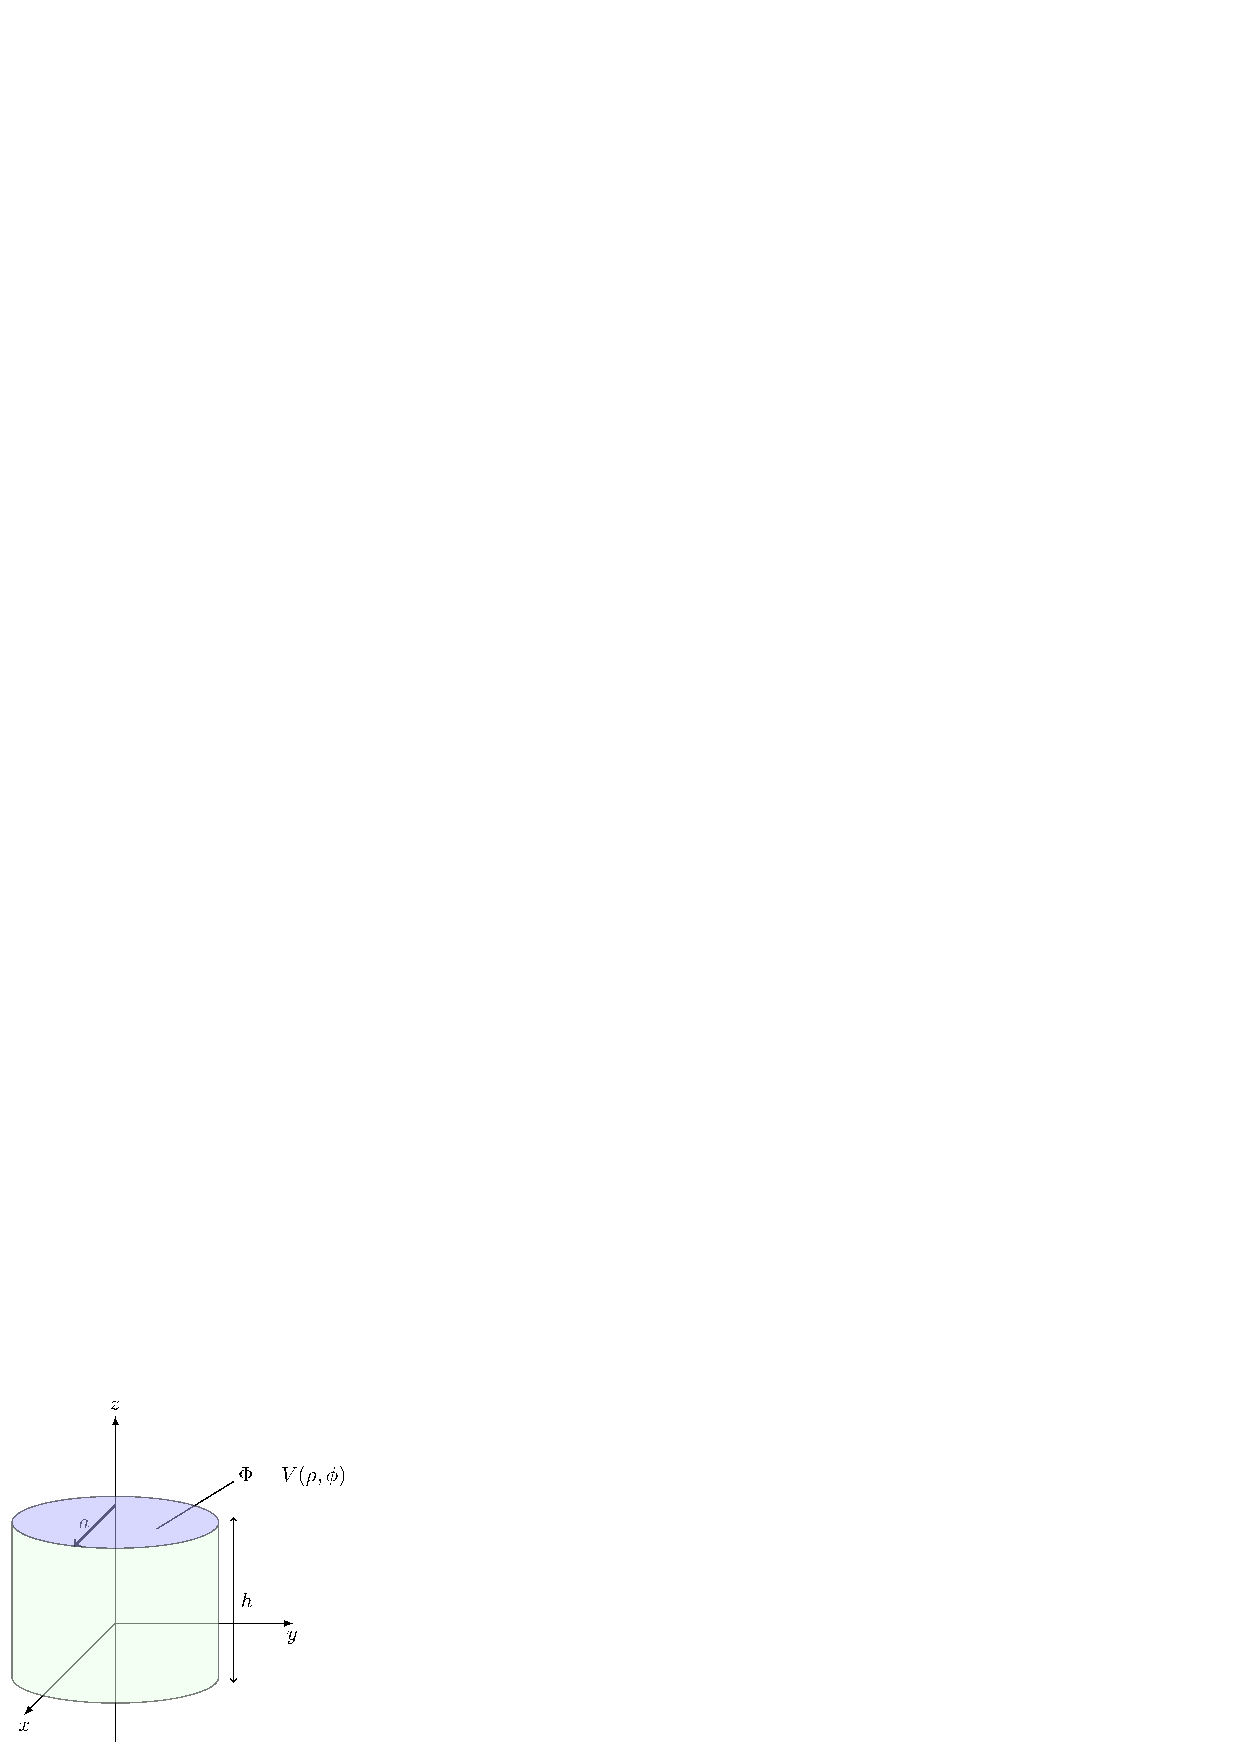
\includegraphics[scale=1.4]{Imagenes/Cilindro_Bessel_01.pdf}
    \caption{Un cilindro conductor que tiene un potencial $V (\rho, \theta)$ en la tapa superior, mientras que el resto de la superficie está aterrizado.}
    \label{fig:figura_27_01}
\end{figure}
Supongamos que el potencial en la tapa superior varía como $V (\rho, \varphi)$ mientras que la superficie lateral y la tapa inferior están conectadas a tierra.
\par
Calculemos el potencial electrostático $\Phi$ en todos los puntos dentro del cilindro.
\par
La solución general es el producto de las soluciones (\ref{eq:ecuacion_27_03}), (\ref{eq:ecuacion_27_04}) y (\ref{eq:ecuacion_27_13}):
\begin{align*}
\Phi (\rho, \varphi, z) = R (\rho) \, S (\varphi) \, Z (z)
\end{align*}
Como $\Phi (\rho, \varphi, 0) = 0$ para cualquier valor arbitrario de $\rho$ y $\varphi$, tenemos que $Z (0) = 0$, dando una constante $Z(z) = \sinh (l \, z)$.
\par
Ya que $\Phi (0, \varphi, z)$ es finito, es finito, no se permite ninguna función de Neumann en la expansión y, dentro de una constante, tenemos $R (\rho) = J_{m}(l \, \rho)$. Además, como $\Phi (a, \varphi, z) = 0$ para cualquier valor arbitrario $\varphi$ y $z$, debemos de tener
\begin{align*}
R (a) = J_{m} (l \, a) = 0 \hspace{0.5cm} \Longrightarrow \hspace{0.5cm} l \, a = x_{mn} \hspace{0.5cm} \Longrightarrow \hspace{0.5cm} l = \dfrac{x_{mn}}{a} \hspace{1cm} n = 1, 2, \ldots
\end{align*}
donde, $x_{mn}$ son las n-ésimas raíces de $J_{m}$.
\par
Ahora podemos multiplicar $R$, $S$ y $Z$ y luego sumar todos los valores posibles de $m$ y $n$, teniendo en cuenta que los valores negativos de $m$ dan términos que dependen linealmente de los valores positivos correspondientes. El resultado es la llamada \textbf{serie de Fourier-Bessel}:
\begin{align}
\begin{aligned}
\Phi (\rho, \varphi, z) &= \nsum_{m=0}^{\infty} \, \nsum_{n=1}^{\infty} J_{m} \left( \dfrac{x_{mn}}{a}  \, \rho \right) \, \sinh \left( \dfrac{x_{mn}}{a}  \, z \right) \times \\[1em]
&\times (A_{mn} \cos m \, \varphi + B_{mn} \sin m \, \varphi )
\end{aligned}
\label{eq:ecuacion_27_39}
\end{align}
donde las constantes $A_{mn}$ y $B_{mn}$ deben ser determinadas por las CDF restantes que establecen que $\Phi (\rho, \varphi, z) = V(\rho, \varphi)$ o
\begin{equation}
V (\rho, \varphi) = \nsum_{m=0}^{\infty} \, \nsum_{n=1}^{\infty} J_{m} \left( \dfrac{x_{mn}}{a}  \, \rho \right) \, \sinh \left( \dfrac{x_{mn}}{a}  \, h \right) \, (A_{mn} \cos m \, \varphi + B_{mn} \sin m \, \varphi )
\label{eq:ecuacion_27_40}
\end{equation}
Multiplicando ambos lados por
\begin{align*}
\rho \, J_{m} \left( \dfrac{x_{mk} \, a}{\rho} \right) \, \cos j \varphi
\end{align*}
para luego integrar de $0$ a $2 \, \pi$, y de $0$ a $a$ en $\rho$, se obtiene $A_{jk}$. Cambiando el coseno al seno, y siguiendo el mismo procedimiento, obtenemos $B_{jk}$. Regresamos del índice $m$ al $n$, por lo tanto
\begin{align}
\begin{aligned}
A_{mn} &= \dfrac{\displaystyle 2 \scaleint{6ex}_{\bs 0}^{2 \pi} \dd{\varphi} \scaleint{6ex}_{\bs 0}^{a} \rho \, V (\rho, \varphi) \, J_{m} \, \left( \dfrac{x_{mn}}{a}  \, \rho \right) \, \cos m \varphi \dd{\rho}}{\pi \, a^{2} \, J_{m+1}^{2} (x_{mn}) \, \sinh \left( \dfrac{x_{mn} \, h}{a} \right) } \\[1em]
B_{mn} &= \dfrac{\displaystyle 2 \scaleint{6ex}_{\bs 0}^{2 \pi} \dd{\varphi} \scaleint{6ex}_{\bs 0}^{a} \rho \, V (\rho, \varphi) \, J_{m} \, \left( \dfrac{x_{mn}}{a}  \, \rho \right) \, \sin m \varphi \dd{\rho}}{\pi \, a^{2} \, J_{m+1}^{2} (x_{mn}) \, \sinh \left( \dfrac{x_{mn} \, h}{a} \right) }
\end{aligned}
\label{eq:ecuacion_27_41}
\end{align}
en donde se ha utilizado la ec. (\ref{eq:ecuacion_27_24}).
\par
El caso importante de simetría azimutal requiere una consideración especial. En tal caso, el potencial de la superficie superior $V (\rho, \varphi)$ debe ser independiente de $\varphi$. Además, como $S (\varphi)$ es constante, su derivada debe anularse. Por lo tanto, la segunda ecuación (\ref{eq:ecuacion_27_01b}) devuelve $\mu = -m^{2} = 0$. Este valor cero de $m$ reduce la suma doble de la ec. (\ref{eq:ecuacion_27_39}) a una sola suma, y obtenemos
\begin{align}
\Phi (\rho, z) = \nsum_{n=1}^{\infty} A_{n} \, J_{0} \left( \dfrac{x_{0n}}{a}  \, \rho \right) \, \sinh \left( \dfrac{x_{0n}}{a}  \, z \right)
\label{eq:ecuacion_27_42}
\end{align}
Los coeficientes $A_{n}$ pueden obtenerse haciendo $m = 0$ en la primera ecuación de (\ref{eq:ecuacion_27_41}):
\begin{align}
A_{n} = \dfrac{4}{a^{2} \, J_{1}^{2} (x_{0n}) \, \sinh \left( \dfrac{x_{0n} \, h}{a} \right)} \, \scaleint{6ex}_{\bs 0}^{a} \rho \, V (\rho) \, J_{0} \, \left( \dfrac{x_{0n}}{a}  \, \rho \right) \dd{\rho}
\label{eq:ecuacion_27_43}
\end{align}
donde $V(\rho)$ es el potencial independiente de $\varphi$ en la tapa superior del cilindro.

\subsection{Cilindro conductor con tapa a un potencial fijo \texorpdfstring{$V_{0}$}{V (0)}.}

Supongamos que la tapa superior de un cilindro conductor se mantiene a un potencial constante $V_{0}$ mientras que la superficie lateral y la tapa inferior están conectadas a tierra. Queremos calcular el potencial electrostático $\Phi$ en todos los puntos dentro del cilindro.
\par
Como el potencial de la tapa superior es independiente de $\varphi$, prevalece la simetría azimutal y la ec. (\ref{eq:ecuacion_27_43}) nos devuelve
\begin{align*}
A_{n} &= \dfrac{4 \, V_{0}}{a^{2} \, \left[ J_{1} (x_{0n}) \right]^{2} \, \sinh \left( \dfrac{x_{0n} \, h}{a} \right)} \, \scaleint{6ex}_{\bs 0}^{a} \rho \,  J_{0} \, \left( \dfrac{x_{0n}}{a}  \, \rho \right) \dd{\rho} \\[1em]
&= \dfrac{4 \, V_{0}}{x_{0n} \, J_{1} (x_{0n}) \, \sinh \left( \dfrac{x_{0n} \, h}{a} \right)}
\end{align*}
donde hemos usado la ec. (\ref{eq:ecuacion_27_18}). El detalle del cálculo de la integral es \textbf{un problema a cuenta}. Se tiene entonces que
\begin{align*}
\Phi (\rho, z) = 4 \, V_{0} \, \nsum_{n=1}^{\infty} \dfrac{J_{0} \left( \dfrac{x_{0n} \, \rho}{a} \right) \, \sinh \left( \dfrac{x_{0n} \, z}{a} \right)}{{x_{0n} \, J_{1} (x_{0n}) \, \sinh \left( \dfrac{x_{0n} \, h}{a} \right)}}
\end{align*}

\section{Problema con distribución de temperaturas.}
\subsection{Geometría del problema.}

Se pide calcular la distribución de temperaturas dentro de un cilindro rígido.
\par
Para iniciar bien la solución de cualquier ejercicio, conviene presentar un esquema del problema. En este caso, el cilindro rígido de radio $r = a$, como vemos en la siguiente figura:
\begin{figure}[H]
    \centering
    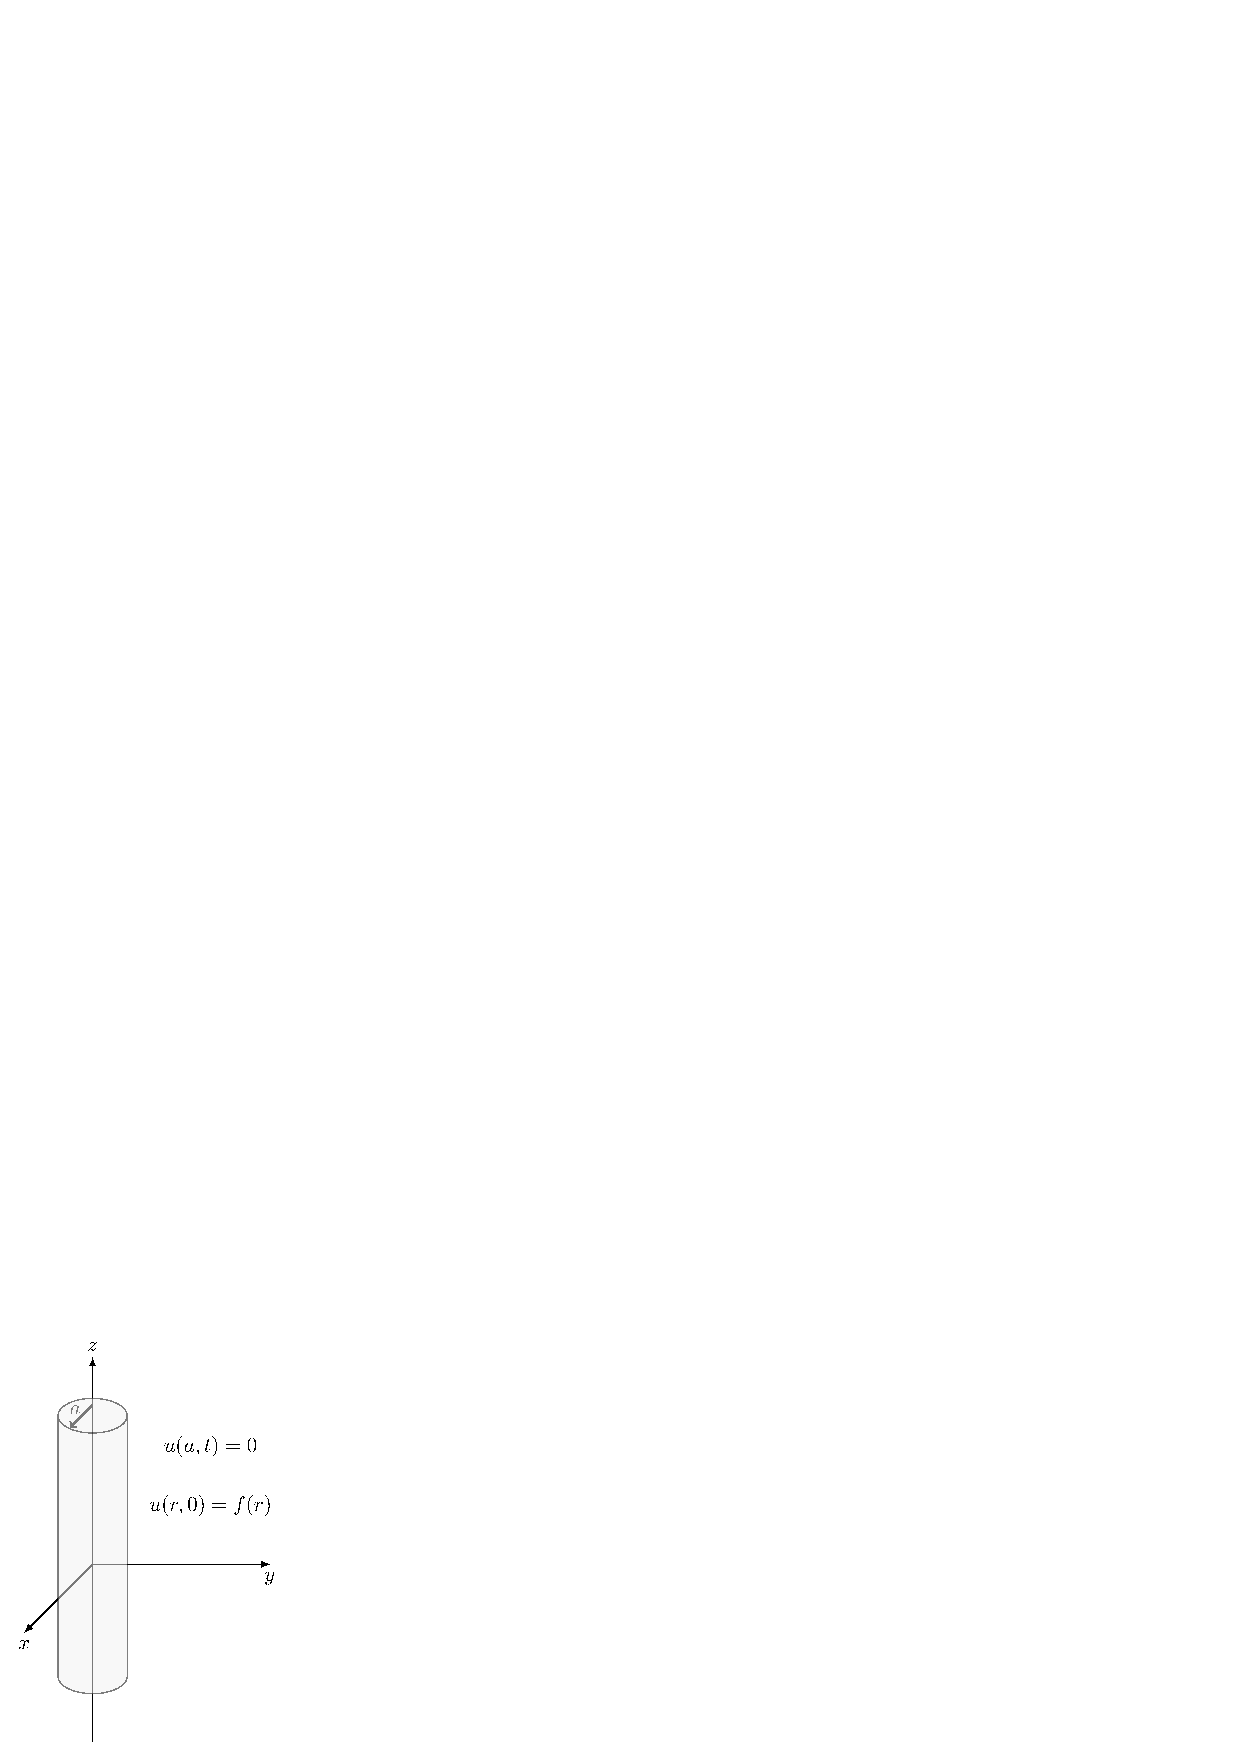
\includegraphics[scale=1]{Figuras/plot_cilindro_Bessel_01.pdf}
\end{figure}
Vemos que no importa la orientación del cilindro, ya sea que lo presentamos de manera horizontal o vertical, el punto importante es considerar que el eje $z$ \enquote{cruza} al cilindro por el centro.

\subsection{Ecuación que modela.}

De acuerdo con lo que nos plantea el enunciado, la ecuación que debemos de ocupar, es la ecuación de calor:
\begin{align}
\pdv{u}{t} = \kappa \left( \pdv[2]{u}{r} + \dfrac{1}{r}  \, \pdv{u}{r} \right) \hspace{1cm} 0 < r < a, \hspace{0.5cm} t > 0
\label{eq:ecuacion_CilBessel_01}
\end{align}
junto con las condiciones:
\begin{align}
u (a, t) = 0 \hspace{2cm} u (r, 0) = f (r)
\label{eq:ecuacion_CilBessel_02}
\end{align}
Debemos de tomar en cuenta que la función $u (r, t)$ (solución) debe de ser acotada en todo el volumen del cilindro.

\subsection{Resolviendo la ecuación.}

Tenemos una EDP lineal y homogénea, por lo que podemos apoyarnos con la técnica de \emph{separación de variables}.
\par
Como la distribución de temperatura no depende  de la parte angular $\theta$, así como del eje $z$, se simplifica el problema. Se propone una solución del tipo:
\begin{align*}
u (r, t) = R (r) \, T (t)
\end{align*}
por lo que se calculan las derivadas parciales $u_{t}$, $u_{r}$ y $u_{rr}$, que vamos a sustituir en la ec. (\ref{eq:ecuacion_CilBessel_01}):
Se tiene entonces que:
\begin{align*}
u_{t} &= R (r) \, \pderivada{T} (t) \\[0.5em] 
u_{r} &= \pderivada{R} (r) \, {T} (t) \\[0.5em] 
u_{rr} &= \sderivada{R} (r) \, {T} (t)
\end{align*}
que se sustituyen en la ecuación de calor.
\par
Ocupando los valores de las derivadas, la ecuación tiene la forma:
\begin{align*}
R (r) \, \pderivada{T} (t) = \kappa \bigg[ \sderivada{R} (r) \, {T} (t) + \dfrac{1}{r} \, \pderivada{R} (r) \, {T}(t) \bigg]
\end{align*}
Esta expresión la dividimos entre $R (r) \, T (t)$:
\begin{align*}
\dfrac{\pderivada{T}}{T} = \kappa \bigg[ \dfrac{\sderivada{R}}{R} + \dfrac{1}{r} \, \dfrac{\pderivada{R}}{R} \bigg]
\end{align*}
simplificamos la expresión:
\begin{align*}
\dfrac{\sderivada{R} + \dfrac{1}{r} \pderivada{R}}{R} = \dfrac{1}{\kappa} \, \dfrac{\pderivada{T}}{T}
\end{align*}
Cada lado de la igualdad depende de una sola variable, al suponer que éstas son independientes entre sí, la única forma en la que se cumple la expresión, es que debe de ser igual a una constante. La constante de separación será: $-\lambda^{2}$.
\par
La ecuación con la constante de separación es:
\begin{align*}
\dfrac{\sderivada{R} + \dfrac{1}{r} \pderivada{R}}{R} = \dfrac{1}{\kappa} \, \dfrac{\pderivada{T}}{T} = -\lambda^{2}
\end{align*}
Debemos de considerar la condición de frontera $u (a, t) = 0$:
\begin{align*}
R (a) \, T (t) = 0 \hspace{1cm} \Rightarrow \hspace{1cm} R (a) = 0
\end{align*}
Llegamos a un sistema de dos EDO2H:
\begin{align}
\sderivada{R} (r) + \dfrac{1}{r} \, \pderivada{R} + \lambda^{2} \, R (r) &= 0, \hspace{1cm} R (a) = 0 \label{eq:ecuacion_CilBessel_03} \\[0.5em]  
\pderivada{T} (t) + \kappa \, \lambda^{2} \, T (t) &= 0 \label{eq:ecuacion_CilBessel_04}
\end{align}

\subsection{La parte radial \texorpdfstring{$R (r)$}{R (r)}.}

La ec. (\ref{eq:ecuacion_CilBessel_03}) que es la parte radial del problema:
\begin{align*}
\sderivada{R} (r) + \dfrac{1}{r} \, \pderivada{R} + \lambda^{2} \, R (r) = 0
\end{align*}
es una ecuación de tipo Bessel:
\begin{align*}
\sderivada{y} + \dfrac{1}{x} \, \pderivada{y} + \left( \lambda^{2} - \dfrac{\nu^{2}}{x^{2}} \right) \, y = 0
\end{align*}
Con $\nu = 0$.
\par
Sabemos que la solución general de la ED de Bessel de orden cero es de la forma:
\begin{align*}
R (r) = C_{1} \, J_{0} (\lambda \, r) + C_{2} \, Y_{0} (\lambda \, r)
\end{align*}
con las constantes $C_{1}$ y $C_{2}$ por determinar, $J_{0}$ es la función de Bessel de primer tipo, mientras que $Y_{0}$ es la función de Bessel de segundo tipo (o funciones de Neumann).

\subsection{Constricciones en el problema.}

La función $R (r)$ debe de estar acotada en $r = 0$,  por lo que se deduce que $C_{2} = 0$, ya que:
\begin{align*}
Y_{0} (0) \to \infty
\end{align*}
Por lo tanto:
\begin{align*}
R (r) = C_{1} \, J_{0} (\lambda \, r)
\end{align*}
como $R (a) = 0$, tenemos:
\begin{align*}
C_{1} \, J_{0} (\lambda \, a) = 0
\end{align*}
Se nos presentan dos casos:
\begin{enumerate}[label=\alph*)]
\item El caso trivial con $C_{1} = 0$.
\item El caso no trivial: $C_{1} \neq 0$, así:
\begin{align}
J_{0} (\lambda \, a) = 0
\label{eq:ecuacion_CilBessel_05}
\end{align}
\end{enumerate}

\subsection{Soluciones a las EDO.}

Si $\lambda_{i} = 1, 2, \ldots$ son las raíces positivas (eigenvalores) de la ec. (\ref{eq:ecuacion_CilBessel_05}), se tiene que aparte del factor constante, las funciones:
\begin{align*}
R_{i} (r) = J_{0} (\lambda_{i} \, r) \hspace{1.5cm} i = 1, 2, \ldots
\end{align*}
son soluciones a la EDO2H radial, ec. (\ref{eq:ecuacion_CilBessel_03}), es decir, son las eigenfunciones.
\par
Para los valores $\lambda$ considerados, la ec. (\ref{eq:ecuacion_CilBessel_04}), es decir, la parte temporal tiene las soluciones particulares:
\begin{align*}
T_{i} (t) = \exp(-\kappa \, \lambda_{i}^{2} \, t) \hspace{1.5cm} i = 1, 2, 3, \ldots
\end{align*}
La sucesión de funciones que son la solución completa:
\begin{align*}
u_{i} (r, t) = C_{i} \, J_{0} (\lambda_{i} \, r) \, \exp(-\kappa \, \lambda_{i}^{2} \, t) 
\end{align*}
satisfacen la ec. (\ref{eq:ecuacion_CilBessel_01}) así como la condición de frontera. De acuerdo con el principio de superposición, la función:
\begin{align}
u (r, t) = \nsum_{i=1}^{\infty} C_{i} \, J_{0} (\lambda_{i} \, r) \, \exp(-\kappa \, \lambda_{i}^{2} \, t)
\label{eq:ecuacion_CilBessel_06}
\end{align}
también satisface a la ecuación de calor inicial y la CDF. Ocupando la condición:
\begin{align*}
u (r, 0) = f (r)
\end{align*}
se obtiene la serie de Fourier-Bessel:
\begin{align}
f (r) = \nsum_{i=1}^{\infty} C_{i} \, J_{0}(\lambda_{i} \, r)
\label{eq:ecuacion_CilBessel_07}
\end{align}
quedando por determinar los coeficientes $C_{i}$.  Para obtener esos coeficientes, haremos un breve repaso sobre las series de Fourier-Bessel.

\subsection{Series de Fourier-Bessel.}

Supongamos que una función $f(x)$ tiene un desarrollo convergente de la forma:
\begin{align}
f (x) = \nsum_{i=1}^{\infty} C_{i} \, J_{\nu} (\lambda_{i} \, x) \hspace{1cm} 0 < x < a
\label{eq:ecuacion_CilBessel_08}
\end{align}
donde los $\lambda_{i}$ con $i = 1, 2, \ldots$ son las raíces positivas de $J_{\nu} (\lambda \, a) = 0$. Multiplicamos ambos lados de la ec. (\ref{eq:ecuacion_CilBessel_08}) por $x \, J_{\nu}(\lambda_{j} \, x)$ con $j$ fijo, para luego integrar entre $0$ y $a$, suponiendo que la serie es integrable término a término, llegando a:
\begin{align*}
\scaleint{6ex}_{\bs 0}^{a} &x \, f(x) J_{\nu}(\lambda_{j} x) \dd{x} = \\[0.5em]
&= \nsum_{i=1}^{\infty} C_{i} \scaleint{6ex}_{\bs 0}^{a} x \, J_{\nu} (\lambda_{i} x) \, J_{\nu} (\lambda_{j} x) \dd{x}
\end{align*}
Para resolver la integral del lado derecho:
\begin{align*}
\scaleint{6ex}_{\bs 0}^{a} x \, J_{\nu} (\lambda_{i} x) \, J_{\nu} (\lambda_{j} x) \dd{x}
\end{align*}
habrá que emplear la propiedad de ortogonalidad de las funciones de Bessel. Sabemos que las funciones de Bessel cuentan con la propiedad de ortogonalidad, dada por la expresión:
\begin{align*}
\scaleint{5ex}_{\bs 0}^{a} &x \, J_{\nu} (\lambda_{i} \, x) \, J_{\nu} (\lambda_{j} \, x) \dd{x} = \\[1em]
&= \begin{cases}
0 & i \neq j \\
\dfrac{a^{2}}{2} \, \big[ J_{\nu+1} (\lambda_{i} \, a)\big]^{2} & i = j, \hspace{0.5cm} i = 1, 2, \ldots
\end{cases}
\end{align*}
Los coeficientes $C_{i}$ son entonces:
\begin{eqnarray*}
\begin{aligned}
C_{i} &= \dfrac{\scaleint{5ex}_{\bs 0}^{a} x \, f(x) \, J_{\nu}(\lambda_{i} \, x) \dd{x}}{\scaleint{5ex}_{\bs 0}^{a} x \, \big[ J_{\nu} (\lambda_{i} \, x) \big]^{2} \dd{x}} \hspace{1cm} i = 1, 2, \ldots \\[1em] 
&= \dfrac{\scaleint{5ex}_{\bs 0}^{a} x \, f(x) \, J_{\nu}(\lambda_{i} \, x) \dd{x}}{\dfrac{a^{2}}{2} \, \big[ J_{\nu+1} (\lambda_{i} \, a) \big]^{2}} \hspace{1cm} i = 1, 2, \ldots
\end{aligned}
\end{eqnarray*}
Por lo tanto, los coeficientes $C_{i}$ quedan definidos por la expresión:
\begin{align*}
C_{i} = \dfrac{2}{a^{2}} \dfrac{\scaleint{5ex}_{\bs 0}^{a} x \, f(x) \, J_{\nu}(\lambda_{i} \, x) \dd{x}}{ \big[ J_{\nu+1} (\lambda_{i} \, a) \big]^{2}} \hspace{1cm} i = 1, 2, \ldots
\end{align*}
Con este resultado, ya podemos regresar al ejercicio y definir la solución completa al problema.

\subsection{Regresando a la solución.}

Con acuerdo a la manera en que se obtuvieron los coeficientes $C_{i}$ de una serie de Fourier-Bessel, para el problema del cilindro, se tiene que:
\begin{align}
\begin{aligned}
C_{i} = \dfrac{2}{a^{2} \, \big[ J_{1} (\lambda_{i} \, a) \big]^{2}} &\scaleint{6ex}_{\bs 0}^{a} r \, f(r) \, J_{0}(\lambda_{i} \, r) \dd{r} \\[0.5em]
i &= 1, 2, \ldots
\end{aligned}
\label{eq:ecuacion_Cil_Bessel_09}
\end{align}
La distribución de temperaturas en el cilindro viene dada por la expresión:
\begin{eqnarray}
\begin{aligned}[b]
u (r, t) &= \dfrac{2}{a^{2}} \nsum_{i=1}^{\infty} \bigg[ \, \scaleint{6ex}_{\bs 0}^{a} \, r \, f(r) J_{0} (\lambda_{i} \, r) \dd{r} \bigg] \, \dfrac{J_{0} (\lambda_{i} \, r)}{\big[ J_{1} (\lambda_{i} \, a) \big]^{2}} \, \exp( -\kappa \, \lambda_{i}^{2} \, t)
\end{aligned}
\label{eq:ecuacion_CilBessel10}
\end{eqnarray}
donde la suma es tomada sobre todas las raíces positivas de la ec. (\ref{eq:ecuacion_CilBessel_05}).

\end{document}